% !TeX root = ../main.tex

\chapter{Thiết kế và triển khai của hệ thống Storm smart home}

Chương này sẽ giới thiệu về mô hình thiết kế và phương pháp triển khai của các thành phần hệ thống sau đây:
\begin{itemize}
    \item Hệ thống Storm smarthome triển khai giữa hệ thống Openstack của trường Công nghệ và hệ thống điện toán đám mây phổ biến AWS.
    \item Hệ thống theo dõi số liệu của mô hình mạng Smarthome và các thông số của các Storm supervisor.
    \item Hệ thống dự đoán tài nguyên trong tương lai.
    \item Hệ thống co dãn Storm supervisor.
\end{itemize}

% \includegraphics[width=0.5\textwidth]{deployment.svg}
\begin{figure}
    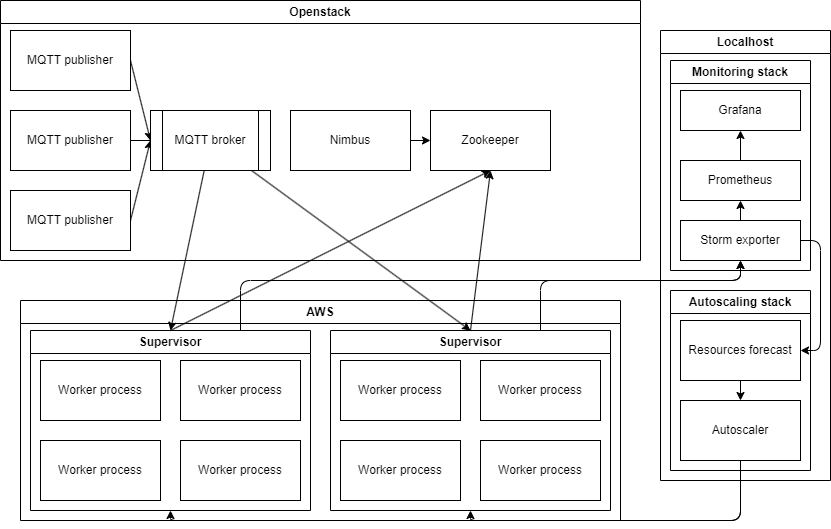
\includegraphics[width=\textwidth]{deployment.png}
    \caption{Sơ đồ toàn bộ hệ thống triển khai}
    \label{}
\end{figure}

\section{Thiết kế}

\subsection{Hệ thống Storm smarthome}

\subsection{Hệ thống tạo dữ liệu của Storm smarthome lên Openstack}

\subsection{Hệ thống xử lý dữ liệu lên AWS}
Hệ thống xử lý dữ liệu bao gồm 4 máy ảo (1 core, 1vCPU) chạy dịch vụ Storm supervisor. Để đơn giản hóa việc triển khai, ta có thể coi việc bật/tắt các dịch vụ Storm supervisor tương đương với việc thêm/xóa các máy ảo chạy dịch vụ Storm supervisor.
Trên các máy ảo này sẽ được cài thêm chương trình \autocite{prometheus_node_exporter} để thu thập các thông số của máy ảo nhằm cung cấp cho prometheus để đánh giá hiệu năng hệ thống và storm-forecast để dự đoán hệ thống.

\subsection{Hệ thống theo dõi số liệu}

\subsubsection{Storm exporter}

Chương trình lấy từ storm topology các thông số về spout, bolt, topology.

\subsubsection{Prometheus}

Thu thập dữ liệu từ storm-exporter, thông số hiệu năng của storm supervisor

\subsubsection{Grafana}

Đồ thị hóa các thông số Prometheus thu thập được.

\subsection{Hệ thống dự đoán tài nguyên}

\subsubsection{Giai đoạn đào tạo}
Trong giai đoạn này, chương trình dự đoán tài nguyên được chạy nhiều lần với các thông số đầu vào là thông số hiệu năng của các Storm supervisor, latency trung bình của topology, spout throughput của hệ thống mạng. Từ các thông số đầu vào, tiến hành dự đoán số lượng máy ảo cần sử dụng trong tương lai, dự đoán này được gửi cho chương trình strom-autoscaler để tiến hành điều chỉnh tài nguyên. Sau khi điều chỉnh tài nguyên và tiến hành tái cân bằng (rebalance) hệ thống mạng, các thông số đầu vào được cập nhật để tiến hành đánh giá hiệu quả. Quá trình lặp lại nhiều lần, mỗi lần trong thời gian 10s để tiến đến mô hình huấn luyện tối ưu. Sau khi kết thúc quá trình huấn luyện, mô hình đã được huấn luyện sẽ được lưu lại và sử dụng trong giai đoạn đánh giá. Mục tiêu của dự đoán là giữ spout throughput, latency của topology, cpu và memory usage của máy ảo ở trong ngưỡng bình thường nhưng đồng thời sử dụng số lượng máy ảo là ít nhất.

\subsubsection{Giai đoạn đánh giá}
Trong giai đoạn này, dựa trên mô hình đã được huấn luyện, ta tiến hành chạy và đánh giá hiệu quả của chương trình với môi trường của các Storm supervisor là máy ảo trong môi trường AWS.

\subsection{Hệ thống co dãn Storm-autoscaler}

\subsubsection{Giai đoạn đào tạo}
Hệ thống là các máy ảo trong môi trường Openstack

\subsubsection{Giai đoạn đánh giá}
Hệ thống là các máy ảo trong môi trường AWS

\section{Triển khai hệ thống}
Do trong môi trường Openstack, các máy ảo được đặt gần nhau hơn rất nhiều so với trong trường hợp các máy ảo được chạy trên hệ thống điện toán đám mây.
Nhằm đảm bảo môi trường mô phỏng là có độ chính xác cao và bám sát với thực tế, ta cần mô phỏng các trường hợp gói tin truyền đi có độ trễ hoặc bị loại bọ trong quá trình truyền.

\subsection{Đo độ trễ trên hệ thống cloud}

Công cụ đo độ trễ được sử dụng là ping\autocite{ping_utility}.

Đo độ trễ giữa supervisor và nimbus. Ta đứng trên host supervisor-1.
\begin{lstlisting}
ping nimbus
\end{lstlisting}

Đo độ trễ giữa các supervisor. Ta đứng trên host supervisor-1.
\begin{lstlisting}
ping supervisor-2
\end{lstlisting}

Tương tự với môi trường trong Openstack. Sau khi thực hiện đo đạc, ta lưu các thông số để thực hiện mô phỏng.

\subsection{Mô phỏng độ trễ}

Để mô phỏng độ trễ của các gói tin hoặc các gói tin bị loại bỏ trong quá trình truyền, ta sẽ sử dụng bộ công cụ \autocite{iproute2}.

Một trong những yếu tố khác nhau tiếp theo giữa môi trường mô phỏng và môi trường thực tế là thời gian khởi động của các nút Storm supervisor. Thông số này có thể dễ dàng tùy chỉnh trong chương trình storm-autoscaler bằng biến môi trường START\_DELAY.

Thời gian xóa bỏ các nút có thể bỏ qua do không có sự khác nhau giữa các cách triển khai.